\section{Semantic Consistency}

The front end language, abstract intermediate language, and the transformation between them 
were designed and implemented together, in order to provide useful abstractions to the user 
and to the tool integrator.  Both languages are specified as layered metamodels 
\cite{mic:overview} which include elements for requirements, design structures, and behavioral 
models.   This translation is similar to the way a compiler translates concrete syntax first 
to an abstract syntax tree, and then to intermediate semantic representations suitable for optimization.
While we do not have space to describe the full
structural and behavioral semantics of the language, Table
\ref{tab:consistencyTools} gives a brief summary of the goals of our
correctness arguments within the full semantics of the language.  The front-end
language, the intermediate language, and the first stage transformation work
together to represent these assumptions and guarantees consistently.

Each analysis translation works from a single view of the design model, keeping 
tool-specific translations simple.  As a simple example, consider the model
shown in Fig. \ref{fig:qr_log_arch}.   Component
DataHandling sends data messages to the other two components, as denoted by the
dependency arrows.  The deployment
view (Fig. \ref{fig:qr_hw_mapping}) shows that each component executes on a
different processor.  Locally, the port object on each component (in both
diagrams) represents the component's view of the actual data message sent over
the wire. The solid connections in the deployment diagram indicate which device
on the processing node will be used to transfer the data.  Specified messages
will participate in processor-local synchronous data flows, or time-triggered
exchanges over the network.  All of these connections and entities are related
to a single semantic message object, which is related to other elements in
different parts of the user model (see the FormattedData message in Fig.
\ref{fig:msg_sched}).  The execution aspect contains timing
information objects, which provide information for fully specifying
the various data transfers.

The first stage transformation checks constraints to ensure that each object is used 
correctly throughout the design, and then reduces this complex set of relations
to a single message object with relations to the other objects that use it. 
Timing parameters from the platform model are used to calculate a behavioral
model for messages and components, including component start times, message 
transfer times, and the duration of each message on the bus.

The passivity of the control components is an interface condition that must be
maintained in order to ensure the proper behavior of the design.  In the user
language we select Simulink subsystems to be used as the specification of
software components in the modeling language.  Each will be implemented as a
synchronous C function.  The selected component objects translate directly to
component instances in the semantic language.  A component is an object with a
unique name (i.e. InnerLoop), and information to find or generate its
implementation in C (in this case, the filename and model path to the Simulink
subsystem "`QuadIntegrator/InnerLoop"'). Though the robustness provided by the
passive abstraction is not yet directly captured in our models, it would be a
more complex concept.  A useful abstraction of the behavior might be the maximum
amount of tolerable time delay on each path (in synchronous time ticks) for the
worst-case input for a particular control loop.  

Note that the language does not currently encode or enforce passive control design 
structure.  However, we require that Simulink models encapsulate functionality 
in subsystem blocks. As passivity is an interface condition, our preservation of
the component structure and synchronous execution semantics should preserve the
passive assumptions of the design, or help designers quickly discover where the
abstraction has broken down.  We will take a look at the validity of our approach 
in Section 9.

\begin{figure}
\centering
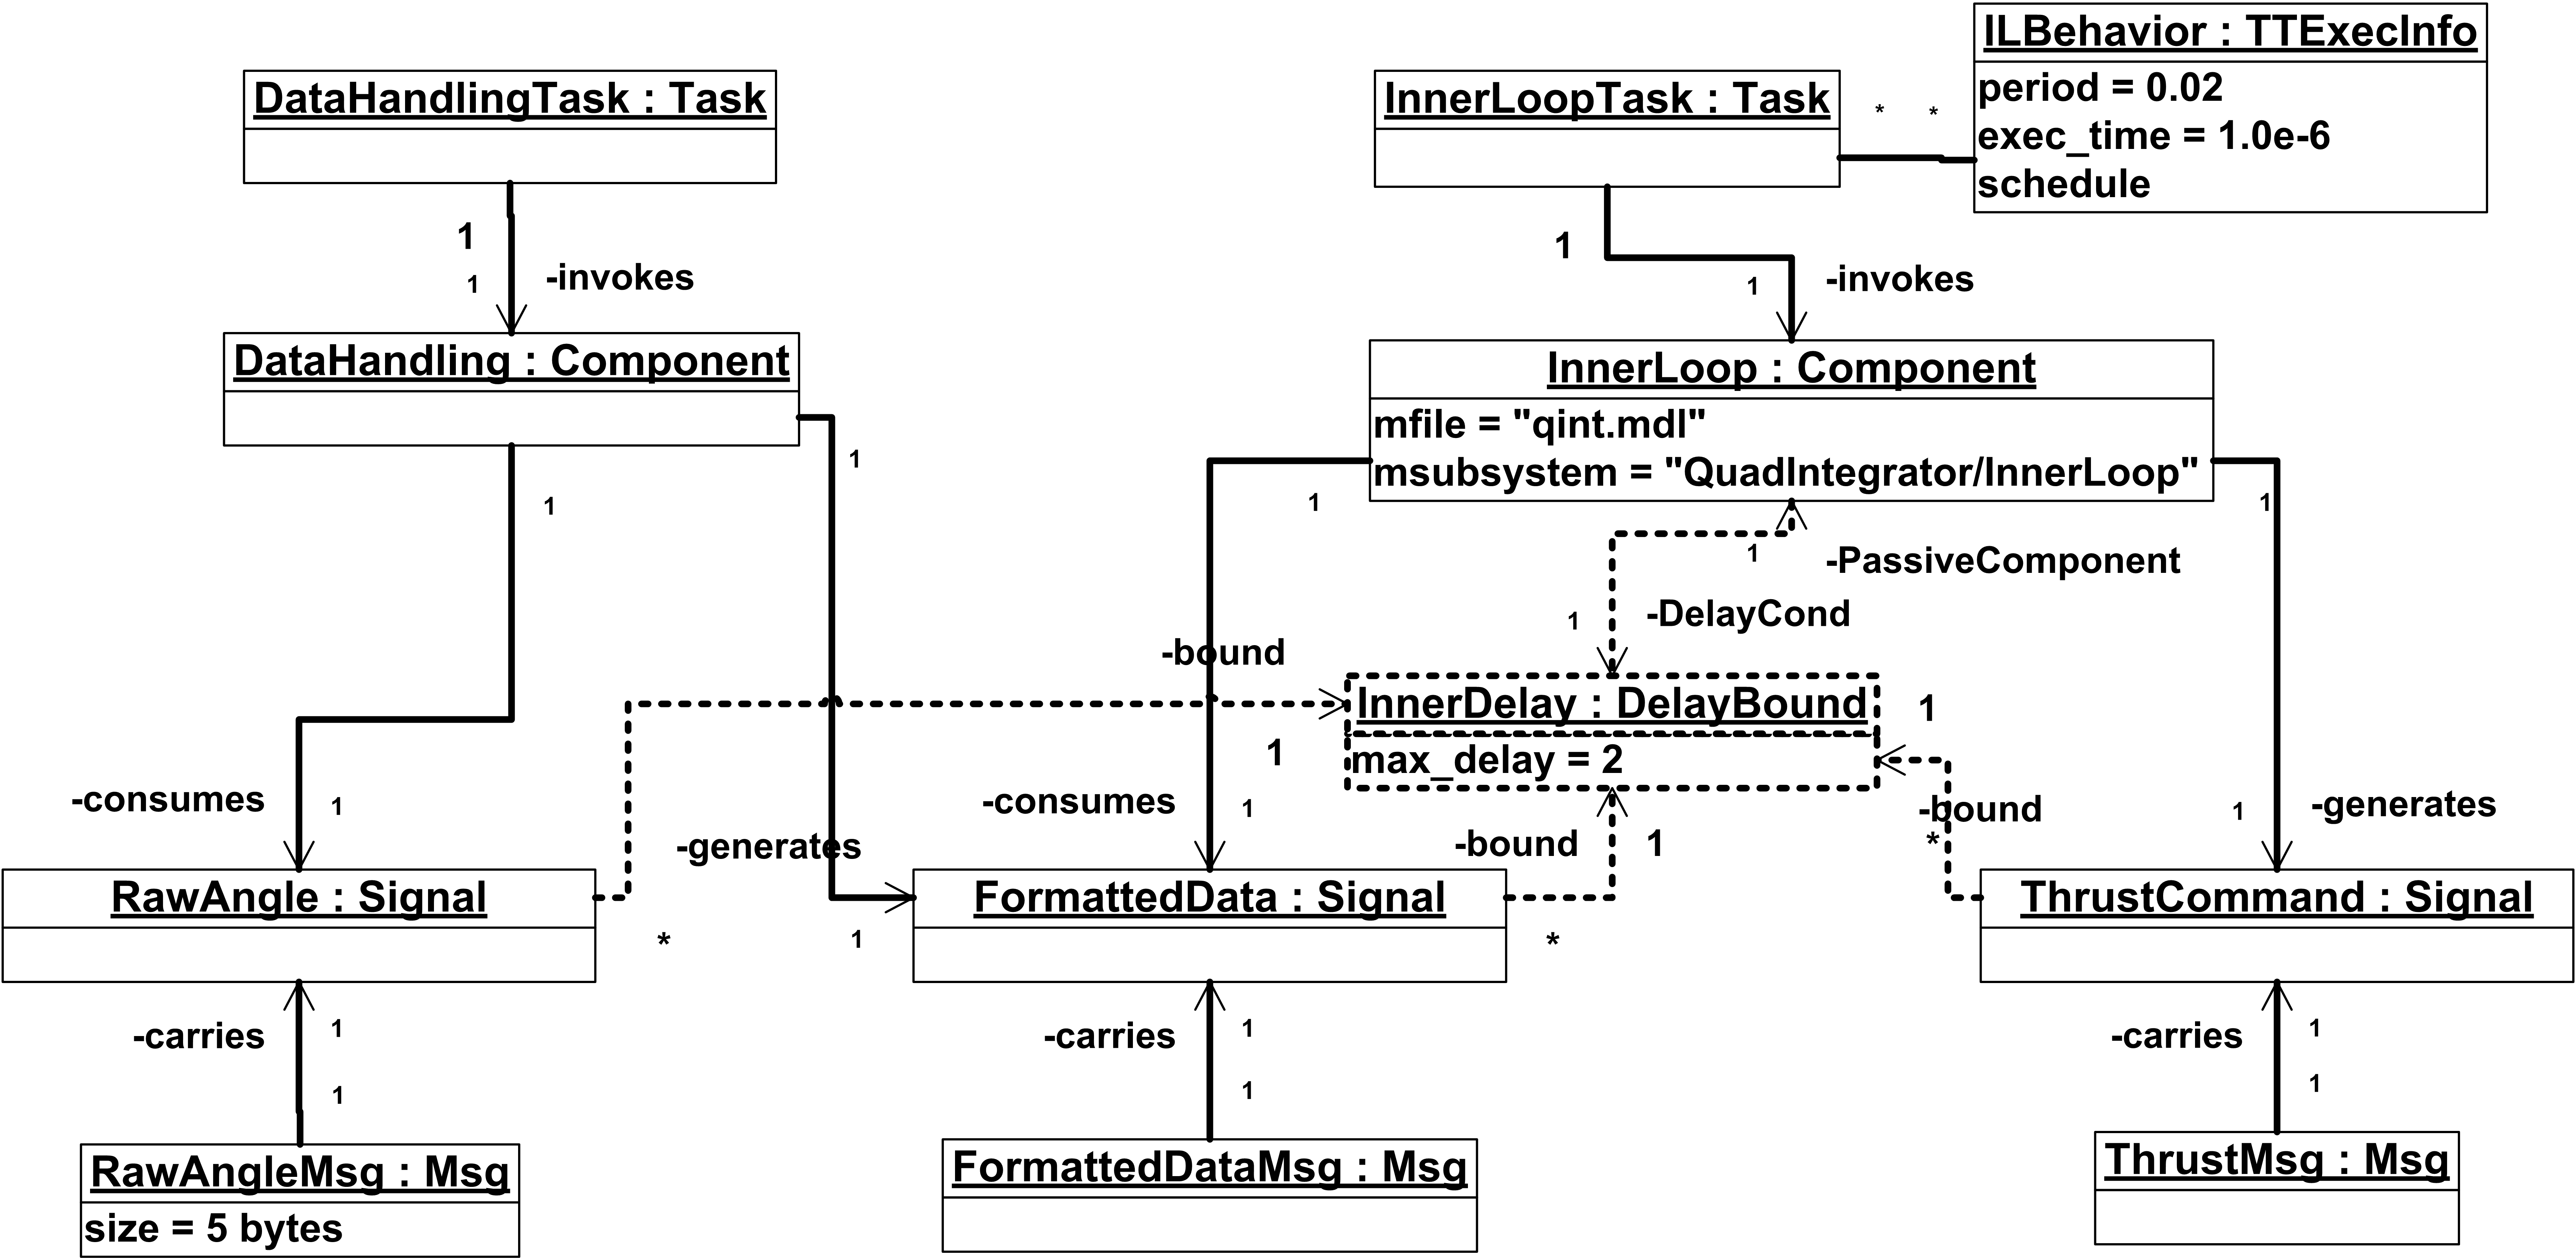
\includegraphics[width=\columnwidth]{figures/delay_bound.png}
    \caption{Capturing a delay bound in the abstract model.  The dashed object
and connectors represent the concept to be represented.  In practice each
high-level design concept or bound is related to many other design objects and
their parameters.}
    \label{fig:delay_abs}
\end{figure}


